% =====================================================================
% 编译说明：本稿含中文红色批注，请在 Overleaf 用 XeLaTeX 编译
% （Menu -> Settings -> Compiler -> XeLaTeX）。定稿投稿前删除所有 \todo{...}。
% =====================================================================
\documentclass[10pt,conference]{IEEEtran}
\IEEEoverridecommandlockouts

% --- Math / symbols ---
\usepackage{amsmath,amssymb,amsfonts}
\usepackage{amsthm}
\usepackage{mathtools}

% --- Graphics, color, tables ---
\usepackage{graphicx}
\usepackage{xcolor}
\usepackage{multirow}
\usepackage{booktabs}
\usepackage{tabularx}
\usepackage{array}
\usepackage{makecell}

% --- Layout / lists / boxes ---
\usepackage{enumitem}
\usepackage{mdframed}
\usepackage[edges]{forest}
\usepackage{pifont}
\usepackage[most]{tcolorbox}
\tcbuselibrary{breakable,listings,skins}

% --- Code rendering ---
\usepackage{listings}
\usepackage{upquote}
\usepackage{seqsplit}
\usepackage[T1]{fontenc}

% --- URLs / hyperlinks ---
\usepackage{url}
\usepackage[hidelinks]{hyperref}
\usepackage{cleveref}

% --- CJK support for the red advisor notes (requires XeLaTeX) ---
%\usepackage{xeCJK}
%用于写批注，后面由于报错，暂时注释掉
% --- Inline code helper ---
\DeclareRobustCommand{\code}[1]{%
  \begingroup
  \ttfamily
  \seqsplit{#1}%
  \endgroup
}
% --- 强行修复 IEEE 引用的特殊控制（紧跟在导言区最后） ---
\makeatletter
\def\cite{\just@cite} % 确保调用 IEEE 原生数字引用
\makeatother
\usepackage{cite}     % 显式加载 IEEEtran 最推荐的 cite 宏包，用于自动实现 [1]-[3] 的连字符压缩
% --- Column types for tables ---
\newcolumntype{Y}{>{\raggedright\arraybackslash}X}
\newcolumntype{C}{>{\centering\arraybackslash}X}
\newcolumntype{L}[1]{>{\raggedright\arraybackslash}p{#1}}
\newcolumntype{M}[1]{>{\centering\arraybackslash}p{#1}}
\newcolumntype{R}[1]{>{\raggedleft\arraybackslash}p{#1}}

% --- Theorem-like environments ---
\newtheorem{definition}{Definition}

% --- Advisor margin notes (rendered red in the PDF; remove before submission) ---
\newcommand{\todo}[1]{\textcolor{red}{\textbf{[TODO]}~#1}}

% --- Robust prompt listing style (used in supplementary material) ---
\lstdefinestyle{promptlisting}{
  basicstyle=\ttfamily\scriptsize,
  columns=fullflexible,
  keepspaces=true,
  showstringspaces=false,
  breaklines=true,
  breakatwhitespace=false,
  breakindent=0pt,
  tabsize=2,
  frame=none,
  numbers=left,
  numberstyle=\tiny\color{gray!65},
  numbersep=0.55em,
  xleftmargin=2.6em,
  resetmargins=true,
  aboveskip=0pt,
  belowskip=0pt,
  prebreak={},
  postbreak={}
}
\newtcblisting[auto counter,number within=section]{PromptBox}[3][]{
  enhanced,
  breakable,
  listing only,
  listing engine=listings,
  listing options={style=promptlisting},
  colback=gray!3,
  colframe=gray!55,
  boxrule=0.4pt,
  arc=1pt,
  left=1.5mm,
  right=1.5mm,
  top=1mm,
  bottom=1mm,
  before skip=6pt,
  after skip=8pt,
  fonttitle=\bfseries\small,
  coltitle=black,
  title={Prompt~\thetcbcounter: #2},
  label={#3},
  #1
}

% --- Anonymized artifact URL placeholder ---
\newcommand{\artifacturl}{\url{https://anonymous.4open.science/r/OH-Bench}}
\newcommand{\codeurl}{\url{https://anonymous.4open.science/r/OH-MAS}}
\begin{document}

\title{OH-MAS: Contracting the Search Space for Static-Analysis Warning Repair}

% Double-blind anonymous submission to ICSE 2027.
\author{\IEEEauthorblockN{Anonymous Author(s)}
\IEEEauthorblockA{Submission to ICSE 2027 -- Double-blind review.}}

\maketitle

\begin{abstract}
Static-analysis linters flag millions of warnings in industrial codebases, and clearing them by hand does not scale. Large language model (LLM) agents promise to automate this, but they are evaluated almost entirely on functional bugs in curated, single-language repositories. On real warnings in heterogeneous, framework-heavy code, such as the OpenHarmony stack that mixes C/C++ and ArkTS, a statically-typed TypeScript dialect, under different linters, conventional agents repair only a minority of cases and incur a high cost for little return. We trace this gap to the structure of the repair loop, not to model capability. An agentic loop makes three decisions and current agents leave all three loose: it edits an unbounded space, often breaking framework invariants; it reacts to failures with free-form reflection that does not accumulate across attempts; and it handles every warning with a single fixed model. OH-MAS makes the three decisions explicit and ties them to one typed signal. A \emph{Repair Contract} bounds the edit space with must-fix locations, must-not-touch invariants, and rule-specific allowed transformations sliced from the project dependency graph. \emph{Typed Diagnostic Feedback} labels each failure as applicability (L1), target-warning (L2), or regression (L3) and accumulates it as constraints that monotonically tighten the contract round by round. A \emph{complementarity-aware model pool} then selects, each round, the models suited to the warning and the last failure. Because the same diagnostic that tightens the contract also widens the pool, repair becomes a bounded search that contracts with every failure rather than a free-form retry. On OH-Bench's 741 real-world OpenHarmony warnings, OH-MAS reaches a 77.9\% strict pass rate, 30.7 points above the strongest agent and 22.0 points above the strongest direct LLM, at \$0.25 to \$0.66 per warning depending on the model pool. A per-mechanism ablation confirms that all three decisions are necessary, with typed diagnostic feedback contributing the largest single gain.
\end{abstract}

\begin{IEEEkeywords}
Automated program repair, static-analysis warnings, large language models, multi-agent systems, OpenHarmony, ArkTS.
\end{IEEEkeywords}

\section{Introduction}

Static analysis is the first line of defense for code quality at industrial scale: every build is scanned for security risks, latent defects, and coding-standard violations. The scan is cheap to run and unforgiving, so a large codebase accrues warnings by the million, far more than developers can triage by hand~\cite{sadowski2015tricorder}. Most are deferred, and the backlog hardens into security and maintenance debt. The cost is highest in the operating systems that ship to hundreds of millions of devices, such as OpenHarmony~\cite{liu2025haptest}, the open-source foundation of HarmonyOS, where a single unresolved warning can block a release or fail a compliance audit. Clearing such a backlog automatically would be of immediate value, and warning repair is unusually well suited to it: unlike a functional bug, every warning names a precise rule, points to an exact location, and arrives with its own machine-checkable oracle, the linter that raised it. A problem this voluminous and this verifiable ought to be the ideal target for automated repair.

It is not, at least not yet: the agents that now resolve a majority of curated functional bugs still clear only a minority of real static-analysis warnings. Automated program repair (APR) has advanced quickly, from generate-and-validate and template-based methods to large language models (LLMs) and, lately, to agents that read a codebase, plan an edit, and revise it from execution feedback~\cite{yang2024swe,zhang2024autocoderover}. That progress, however, is measured almost entirely on benchmarks of single-language, well-isolated repositories such as SWE-bench~\cite{jimenez2024swe} and Defects4J~\cite{just2014defects4j}, not on the heterogeneous, framework-heavy, repository-scale code that dominates industry. The shortfall is not a shortage of model capability; it is the loose structure of the repair loop wrapped around the model.

That looseness has a precise anatomy: beneath their surface differences, all repair loops perform one task, searching a space of candidate edits for one the verifier will accept, and three decisions govern how a loop traverses that space. We call this space the loop's \emph{search space}; the three decisions are which edits it contains, what the loop learns from a rejected attempt, and which model proposes the next candidate. Today's agents, from SWE-agent~\cite{yang2024swe} and Agentless~\cite{xia2025demystifying} to RepairAgent~\cite{bouzenia2025repairagent} and AutoCodeRover~\cite{zhang2024autocoderover}, leave all three implicit, and each omission carries a concrete cost.
\textbf{The edit space is unbounded.} The agent may rewrite any line, so it routinely breaks an invariant the surrounding code silently relies on, such as a public signature or a framework decorator.
\textbf{The failure signal is untyped.} A rejected patch returns as raw text and is met with free-form reflection, so ``it did not apply,'' ``it did not remove the warning,'' and ``it introduced a new defect'' are treated alike, and a diagnosis made in one round is forgotten in the next.
\textbf{The generator is a single model.} One backbone handles every warning, although no single model is strongest across rule families and language layers.
The three weaknesses compound rather than cancel: an unbounded space breeds more failures, untyped feedback fails to learn from them, and a single model cannot see past its own blind spots. This is why a bigger model does not close the gap.

The remedy is to make the three decisions explicit and, just as important, to couple them through one signal. Bound the edit space before generation; type every failure so that it permanently narrows that space; and choose the model per warning. The power lies in the coupling. A single typed failure can serve twice, tightening the bound on what may be edited and selecting which model edits next, so each rejection leaves the next attempt both smaller and better aimed. Free-form generation thereby becomes a search that contracts with every failure, the discipline that counterexample-guided abstraction refinement~\cite{clarke2000cegar} brought to verification.

We instantiate and evaluate this design on OpenHarmony, the setting that stresses all three decisions at once. Its codebase is deeply heterogeneous: C/C++ system code and ArkTS application code, the latter a statically-typed TypeScript dialect for declarative UI, coexist under different linters and rule families, so neither a single edit space nor a single model fits both. Its framework code obeys invariants, such as the lifecycle callbacks and reactive-state decorators of ArkUI (OpenHarmony's declarative UI framework), that a general-purpose model has seldom seen and easily violates, and its engineering roadmap names automated defect repair as a priority~\cite{li2025software}. Benchmarking on its repositories~\footnote{\url{https://anonymous.4open.science/r/OH-Bench}} points to the same three decisions from the data side: structural retrieval over project dependencies far outperforms text-similarity retrieval; repair competence stratifies into format, semantics, and regression-freedom; and no single model dominates across rule families and language layers. The one prior OpenHarmony repair system, HapRepair~\cite{lin2025haprepair}, pairs CodeLinter (OpenHarmony's official ArkTS static analyzer) with retrieval-augmented generation (RAG), but it addresses none of these decisions and handles ArkTS alone.

We present \textbf{OH-MAS} (OpenHarmony Multi-Agent System), a four-stage repair system that makes the three decisions explicit and drives them from one typed evidence stream. Three agents, an \emph{Adaptive Orchestrator}, a \emph{Graph Weaver}, and a \emph{Constrained Patcher}, are closed by a deterministic \emph{Diagnostic Auditor}. The resulting loop is a bounded search that tightens with every failure instead of restarting from scratch. Three mechanisms, one per decision, realize it:

\begin{itemize}

    
\item \textbf{Bound the space with a Repair Contract.} The Graph Weaver slices the project dependency graph into a typed triple: \emph{must-fix} locations, \emph{must-not-touch} invariants (public signatures, framework decorators, cross-file types), and rule-specific \emph{allowed transformations}. The Constrained Patcher may act only inside this triple, which turns free-form completion into constraint-satisfaction within a bounded space. The contract follows the spirit of Design by Contract~\cite{meyer1992dbc}: it states what the patcher must fix and what it must preserve.

\item \textbf{Contract the space with Typed Diagnostic Feedback.} The Diagnostic Auditor labels every failure as applicability (L1), target-warning (L2), or regression (L3). The Orchestrator turns each label into a hard constraint and never discards it, so the constraint set only grows from one round to the next and each new round searches within the space the previous one left open.

\item \textbf{Match the generator with a complementarity-aware pool.} The same typed signal selects, each round, a subset of a heterogeneous model pool and widens it as the difficulty rises, so model complementarity becomes a first-class input rather than a post-hoc majority vote.
\end{itemize}
The three mechanisms reinforce one another: the diagnostic that tightens the contract is the same signal that widens the pool, and the contract bounds what every pooled model may do. Constraint-based repair, monotonic contracting, and model routing each address one axis alone; to our knowledge no prior repair system makes all three explicit and couples them through a single typed signal. A pre-built dependency graph and rule-specialized templates from concurrent work (hosted under the \texttt{/oh-kb} subdirectory of the same repository) are swappable inputs, not contributions of this paper.



\begin{table}[t]
\centering
\caption{Where representative repair systems stand on the three decisions a repair loop must make explicit: a bounded edit space, a typed failure signal that contracts it, and an instance-matched generator. ``Partial'' marks a channel structured at the file or function level that carries no hard prohibitions or invariants.}
\label{tab:comparison}
\vskip -0.05in
\resizebox{\columnwidth}{!}{%
\begin{tabular}{lcccc}
\toprule
System & Bounded space & Typed feedback & Multi-model & Target domain \\
\midrule
SWE-agent~\cite{yang2024swe}            & $\times$    & $\times$    & $\times$    & Python (SWE-bench) \\
Agentless~\cite{xia2025demystifying}            & partial     & $\times$    & $\times$    & Python (SWE-bench) \\
RepairAgent~\cite{bouzenia2025repairagent}   & $\times$    & $\times$    & $\times$    & Java (Defects4J) \\
AutoCodeRover~\cite{zhang2024autocoderover}  & partial     & $\times$    & $\times$    & Python / Java \\
HapRepair~\cite{lin2025haprepair}            & $\times$    & $\times$    & $\times$    & ArkTS only \\
\midrule
\textbf{OH-MAS} (ours)                       & \checkmark  & \checkmark  & \checkmark  & C/C++ + ArkTS \\
\bottomrule
\end{tabular}
}
\vskip -0.1in
\end{table}

On OH-Bench, a repository-level benchmark of 741 real-world warnings (382 ArkTS, 359 C/C++), making the three decisions explicit turns a divergent loop into a convergent one. OH-MAS reaches a \textbf{77.9\%} strict pass rate, ahead of the strongest agent (Moatless) by \textbf{30.7} percentage points (pp) and the strongest direct LLM (Claude Opus 4.8) by \textbf{22.0}~pp, and it improves both the ArkTS (81.4\%) and C/C++ (74.1\%) layers, at \$0.25 to \$0.66 per warning. A per-mechanism ablation confirms that all three are necessary, with typed diagnostic feedback contributing the largest single gain.

Our key contributions are as follows:
\begin{itemize}
\item \textbf{A reframing of warning repair.} We cast warning repair as a search for an oracle-accepting edit and identify the three decisions every repair loop makes but today's agents leave implicit: the edit space it may explore, what it learns from each rejected attempt, and which model proposes the next edit.
\item \textbf{A coupled instantiation, OH-MAS.} We realize the three decisions from one typed evidence stream: \emph{Repair Contracts} bound the space, \emph{Typed Diagnostic Feedback} (L1/L2/L3) contracts it monotonically so the admissible edit set never grows across rounds, and a \emph{complementarity-aware} pool supplies the generator. The same diagnostic that tightens the contract also widens the pool. We know of no prior repair system that couples these three through a single typed signal.
\item \textbf{Evidence on OpenHarmony.} On a repository-level benchmark spanning C/C++ and ArkTS, OH-MAS reaches 77.9\% strict pass rate and outperforms twelve baselines by 30.7~pp over the strongest agent. A per-mechanism ablation, a per-language sub-analysis, a cost-effectiveness breakdown, and a per-round measurement of the contracting search space show that each decision is necessary.
\end{itemize}
This paper gives background and a motivating example (\S\ref{sec:background}), details the architecture (\S\ref{sec:approach}), reports the evaluation (\S\ref{sec:evaluation}), and discusses implications, threats, and related work (\S\ref{sec:discussion}--\ref{sec:related}).

\section{Background and Motivation}
\label{sec:background}

\subsection{Autonomous Agents in Program Repair}
\label{sec:bg_apr}

LLM agents have displaced template-based heuristics as the dominant paradigm for APR~\cite{xia2025demystifying}. Systems such as SWE-agent~\cite{yang2024swe} and AutoCodeRover~\cite{zhang2024autocoderover} model repair as an interactive loop: an agent reads the codebase, plans a fix, edits files through an Agent-Computer Interface (ACI), and observes feedback from the environment. These frameworks do well on homogeneous, single-language benchmarks (e.g., SWE-bench for Python), but they rest on one implicit assumption: that the agent already knows enough to infer the structural invariants it must not break. Their action space therefore stays unbounded, and recovery from a failed edit falls back on open-ended natural-language reflection.

\subsection{Repairing Heterogeneous Ecosystems}
\label{sec:bg_oh}

Industrial operating systems break the assumptions of unconstrained agents, and OpenHarmony is a sharp example. It interleaves low-level C/C++ system components with ArkTS application code, each governed by its own linter and rule family. Repairing static-analysis warnings here raises two challenges that single-language agents never confront.

\textit{Framework invariants restrict valid edits.} Framework code such as ArkUI components is governed by strict lifecycle callbacks and reactive state decorators (e.g., \texttt{@State}, \texttt{@Link}). These contracts are framework-specific and rarely appear in general-purpose LLM pre-training corpora, so a model cannot reliably infer them.

\textit{Local defects have non-local causes.} A warning that looks local often stems from a violation of inter-procedural or cross-file data flow. Editing the flagged abstract syntax tree (AST) node without tracing its dependencies tends to trigger cascading violations in components that looked unrelated. Both challenges point the same way: similarity-based RAG is not enough, because the agent needs explicit, deterministic structural boundaries to keep its edits from hallucinating dependencies.

\subsection{A Motivating Example of Agent Failure}
\label{sec:bg_motivating}

A single warning is enough to expose the fragility of an unbounded loop. Consider a \texttt{hp-arkui-use-reusable-component} violation in an ArkTS application: the linter flags a \texttt{LazyForEach} loop for inefficient rendering, and a correct fix must extract the child component, add a \texttt{@Reusable} decorator, and pair it with an \texttt{aboutToReuse()} lifecycle method that re-binds state on reuse. A general-purpose agent that processes this warning slides into a divergent trajectory in three phases.

\textbf{Phase 1, destructive edit.} The agent locates the child component but, without explicit knowledge of the framework's invariants, adds the \texttt{@Reusable} decorator and omits the mandatory state-synchronization logic.
\textbf{Phase 2, cascading regression.} The patch is valid ArkTS, so the linter accepts the decorator change (an L1 applicability success). A repository-wide scan then reports a new defect: the reused component now captures dynamic external state, violating the reuse contract. Because the feedback is untyped, the agent cannot separate this regression (an L3 outcome) from the fact that the patch did apply cleanly, so it cannot tell a promising partial fix from a dead end.
\textbf{Phase 3, divergent reflection.} The environment returns a raw error log. Unable to link the regression to its earlier omission, the agent reflects by inventing a mock state object or deleting the loop outright, which deepens the damage. The agent is also locked to one backbone, so even if another model understood ArkTS reuse semantics, the loop could not call on it.

The same example exposes all three loose decisions at once: the agent edits an unbounded space, receives undifferentiated feedback that does not accumulate, and is tied to a single model. The next subsection turns these into design imperatives, and Section~\ref{sec:app_walkthrough} returns to this exact warning to show OH-MAS converging where the unbounded loop diverged.

\subsection{Design Imperatives}
\label{sec:bg_imperatives}

The example shows that closing the gap between autonomous repair and heterogeneous code calls for structural intervention on each loose decision. We state three imperatives that define the OH-MAS architecture.

\begin{enumerate}[label=\textbf{I\arabic*.}, leftmargin=*, topsep=2pt, itemsep=4pt]
    \item \textbf{Bound the edit space.} Replace heuristic context retrieval with a deterministic \emph{Repair Contract} that names the \emph{must-fix} nodes and the \emph{must-not-touch} invariants by slicing the dependency graph, so destructive edits are ruled out before generation.
    \item \textbf{Type and accumulate the failure signal.} Project every failure into a typed, hard constraint that monotonically shrinks the search space for later rounds, so the loop converges instead of oscillating on free-form reflection.
    \item \textbf{Match the model to the instance.} Route each round to a heterogeneous pool of models rather than one backbone, trading search breadth against token cost as difficulty rises.
\end{enumerate}

\section{Approach: The OH-MAS Architecture}
\label{sec:approach}

We formalize automated warning repair as a state-machine-driven constraint-satisfaction problem. Given a codebase $\mathcal{V}$ and a static-analysis warning $w = \langle f, \ell, r, m \rangle$ (comprising the file path, line span, rule identifier, and message), the objective is to synthesize a patch $p$ that satisfies a deterministic verification oracle $\mathcal{O}(p, \mathcal{V}) \to \text{Pass}$ within a bounded computational budget. OH-MAS realizes this objective with the same three mechanisms introduced above: it bounds the edit space with Repair Contracts (\S\ref{sec:app_gw}), contracts that space monotonically with Typed Diagnostic Feedback (\S\ref{sec:app_refinement}), and matches the generator to the instance with a complementarity-aware model pool (\S\ref{sec:app_routing}).

\subsection{System Overview}
\label{sec:app_overview}

OH-MAS runs repair as a four-stage loop that keeps the edit space bounded at every step. Figure~\ref{fig:overview} illustrates the components and the typed signal linking them.

\begin{figure}[t]
  \centering
  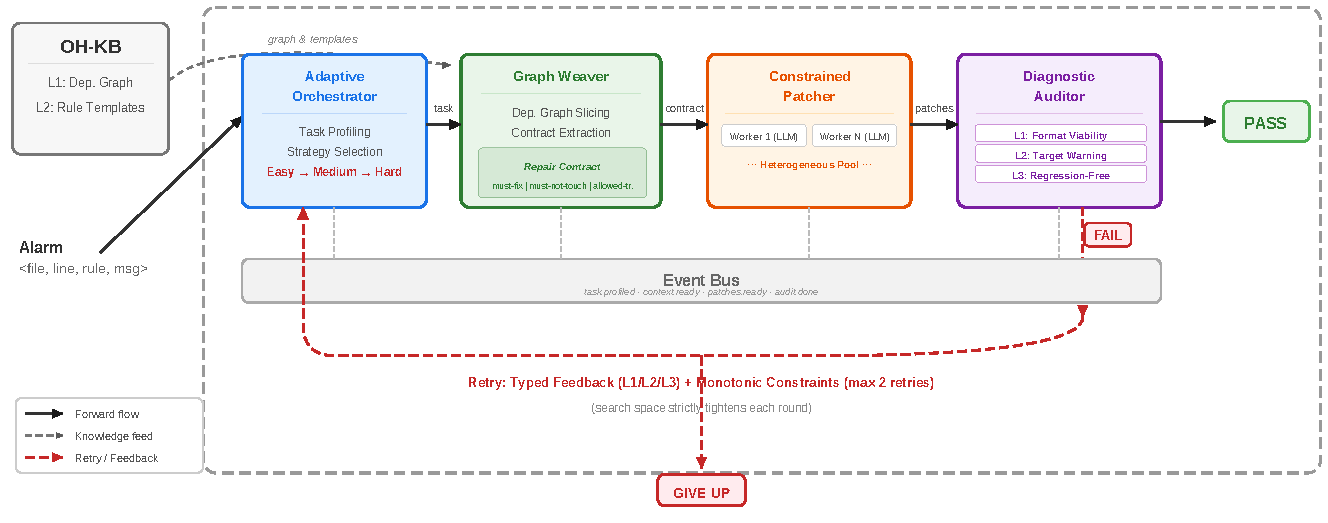
\includegraphics[width=\columnwidth]{overview.pdf}
  \caption{Overview of OH-MAS. The \textbf{Adaptive Orchestrator (AO)} profiles the warning and sets the execution mode. The \textbf{Graph Weaver (GW)} slices the dependency graph to extract a \emph{Repair Contract} comprising must-fix locations, must-not-touch invariants, and allowed transformations. The \textbf{Constrained Patcher (CP)} generates patches within this contract using a heterogeneous model pool. The deterministic \textbf{Diagnostic Auditor (DA)} validates candidates across three hierarchical tiers: applicability (L1), target-warning (L2), and regression (L3). Failed audits return typed evidence, which the AO accumulates as monotonically tightening constraints for the next round.}
  \label{fig:overview}
\end{figure}

The \textbf{Adaptive Orchestrator (AO)} serves as the central state controller. In the first round ($t{=}0$), it operates in \emph{Easy} mode: it profiles the warning's language layer and rule category, and dispatches the task to a single pre-configured model.

The AO then invokes the \textbf{Graph Weaver (GW)}, which performs deterministic graph slicing to emit a \emph{Repair Contract}. This structured artifact defines the permissible edit space: the exact locations to fix, the structural invariants to preserve, and rule-specific transformation templates. In Easy mode, the slice captures only local context; as modes escalate, the GW expands the cross-file scope and injects richer invariants.

The contract goes to the \textbf{Constrained Patcher (CP)}, which queries a heterogeneous pool of LLMs for candidate patches that stay inside the contract. The \textbf{Diagnostic Auditor (DA)} then checks each candidate in an isolated sandbox across three tiers: applicability (L1), target-warning elimination (L2), and regression freedom (L3).

A failed audit drives the next round. Rather than triggering unstructured natural-language reflection, the AO parses the DA's typed failure report into persistent hard constraints, escalates the execution mode (Easy $\rightarrow$ Medium $\rightarrow$ Hard), and routes the prompt to a wider set of models. Each retry therefore searches within the sub-space left open by the previous round. OH-MAS splits labor between LLM reasoning and deterministic control: the orchestrator and weaver use an LLM to interpret the warning and its sliced context, but the decisions that bound the search, the graph slice, the round-to-round routing, and the three-tier audit, are computed by fixed rules, which is what makes the contract a hard boundary rather than a suggestion.

\subsection{Bounding the Space: Graph Weaving and Repair Contracts}
\label{sec:app_gw}

The bottleneck in repository-level repair is context pollution: raw source files exceed optimal context windows, and heuristic semantic retrieval frequently pulls in code that violates compilation boundaries. The Graph Weaver (GW) avoids both by replacing retrieval with deterministic graph slicing, outputting a typed \emph{Repair Contract} $\mathcal{C}_w$ that formally bounds what the patcher is allowed to do.

\textbf{Contract structure.} We model the repository as a directed dependency graph $\mathcal{G} = (V, E)$, where vertices denote structural code elements and edges denote compile-time relations. Given a warning $w$, the GW runs a rule-specific traversal to extract a contextual subgraph, formalizing $\mathcal{C}_w$ as a typed triple:

\begin{enumerate}[label=\textbf{(M\arabic*)}, leftmargin=*, topsep=2pt, itemsep=4pt]
\item \textbf{Must-fix locations}: The minimal lexical block enclosing the defect span $\ell$ (e.g., an ArkUI component definition or a C++ function body), tagged with its structural role.
\item \textbf{Must-not-touch invariants}: Explicit assertions the patch must preserve, derived from $\mathcal{G}$ (e.g., cross-file type dependencies, public API signatures, and framework decorators). This establishes a strict information boundary against LLM hallucination.
\item \textbf{Allowed transformations}: Rule-keyed repair templates retrieved from an offline knowledge base. They encode the intended syntactic structure of the fix (e.g., ``insert a null-guard before the dereferenced pointer'').
\end{enumerate}

This triple converts patch generation from an open-ended text completion task into a constraint-satisfaction problem: the patcher sees only the must-fix region, cannot alter a must-not-touch invariant, and is steered by allowed transformations. 

\textbf{Depth scales with difficulty.} The execution mode sets the slicing depth. In Easy mode ($t{=}0$), the GW takes a local 1-hop slice and injects basic invariants, keeping a trivial formatting fix economical. After a failure, in Medium and Hard modes, it widens to a 2-hop slice and enriches the must-not-touch set with decorator metadata and inter-procedural data-flow edges, giving a cross-file refactoring the structural depth it needs.

\subsection{Contracting the Space: Hierarchical Auditing and Monotonic Refinement}
\label{sec:app_refinement}

A bounded space is not enough; the loop must learn from intermediate failures. Conventional autonomous agents feed raw error output back to the LLM, which invites hallucinated fixes and an oscillating trajectory. OH-MAS instead routes every failure through a typed, hierarchical audit.

The Diagnostic Auditor (DA) checks a candidate patch $p_t$ in three discrete tiers. \textbf{L1 Applicability} asks if $p_t$ is a syntactically valid unified diff. \textbf{L2 Target-Warning} queries the static analyzer to confirm the elimination of $w$, returning the residual warning locations $\Delta_{res}$ if it fails. \textbf{L3 Regression} runs a repository-wide differential scan and returns the regression context $\Delta_{reg}$ if the patch introduces a secondary defect $w_{new}\notin W(\mathcal{V})$, that is, a warning absent from the codebase's original warning set $W(\mathcal{V})$. The DA stops at the lowest failing tier, keeping the error signal causally isolated.

Each typed verdict becomes a permanent constraint on the next round, which we now make precise. Let $\Omega_t$ be the set of patches the patcher is still allowed to propose at round $t$, that is, the patches consistent with the contract $\mathcal{C}_w$ and with the history $\mathcal{H}_t$ of constraints accumulated so far:
\begin{equation}
\label{eq:contract}
    \Omega_t = \{\, p : p \models \mathcal{C}_w \ \wedge\ p \models \mathcal{H}_t \,\}.
\end{equation}
The AO turns each typed failure into a constraint and never discards it. It maps the failure report $\mathcal{F}_t$ into a constraint payload $e_{t+1}$ that carries the exact residual evidence, and appends it to the history, $\mathcal{H}_{t+1} = \mathcal{H}_t \cup \{e_{t+1}\}$, so the next prompt is the contract concatenated with the history, $P_{t+1} = \mathcal{C}_w \oplus \mathcal{H}_{t+1}$. Because each round only adds conjuncts and never removes one, the admissible space is non-increasing,
\begin{equation}
\label{eq:monotone}
    \Omega_{t+1} \subseteq \Omega_t .
\end{equation}
This is exactly what free-form reflection lacks: a rejected patch there leaves the next attempt free to revisit the same region, so the trajectory can oscillate. Under monotonic accumulation, the loop instead searches within the previous round's space, which is why later rounds converge and cost less.

Two qualifications keep this guarantee honest. First, Eq.~\eqref{eq:contract} fixes the contract $\mathcal{C}_w$, so the containment in Eq.~\eqref{eq:monotone} holds at a fixed slicing scope; mode escalation is the one controlled exception, in which the GW widens its slice to admit cross-file edits the earlier scope excluded and so restores reachability when the accumulated constraints would otherwise leave $\Omega_t$ empty. Even then the widening stays bounded by the dependency graph and still enforces every must-not-touch invariant, so it re-bounds the search rather than reopening the whole file as free-form reflection does. Second, monotonic contracting guarantees non-divergence, not completeness: it cannot manufacture a valid patch when none lies in $\Omega_t$, and an over-tight history could in principle exclude every fix, which is why escalation pairs each tightening with a wider slice and a stronger pool. Section~\ref{sec:rq3_result} reports the observable footprint this contraction leaves in practice.

\subsection{Matching the Generator: Dynamic Model Pooling}
\label{sec:app_routing}

C/C++ memory semantics and ArkTS reactive state demand different reasoning, and no single model is best at both. OH-MAS therefore drops the static backbone and gives the Constrained Patcher a heterogeneous pool $\Theta = \{\theta_1, \dots, \theta_k\}$. The AO acts as a rule-based meta-controller that, each round, sends the prompt to a subset $\Theta_t \subseteq \Theta$ chosen according to deterministic heuristics.

\textbf{First attempt.} At $t{=}0$ there is no failure to learn from, so the AO routes to a single model pre-configured for the warning's language and category. This is the cost-effective exploration baseline.

\textbf{After a failure.} For $t>0$, the AO applies a deterministic routing policy keyed on four metadata signals: the rule category, the language layer (ArkTS or C/C++), the current mode, and the failure tier (L1, L2, or L3). From these it selects $\Theta_t$ and, when the diagnostic indicates a complex semantic failure, spawns several CP workers that run different models in parallel; the first to reach a Pass halts the rest. Compute thus grows with difficulty rather than being spent uniformly.

\subsection{The Repair Loop on the Motivating Example}
\label{sec:app_walkthrough}

The three mechanisms are clearest when traced together on the warning that defeated the unconstrained agent in Section~\ref{sec:bg_motivating}. We follow OH-MAS on the same \texttt{hp-arkui-use-reusable-component} instance: a \texttt{LazyForEach} loop must become a reusable child component that carries a \texttt{@Reusable} decorator and an \texttt{aboutToReuse()} method to re-bind state on reuse. Where the baseline agent oscillated, OH-MAS converges after one typed failure.

\textbf{Round $t{=}0$ (Easy mode).} The AO profiles the warning as an ArkTS component-performance rule and dispatches it to a single pre-configured model, keeping the common case cheap. The GW extracts a 1-hop slice from the file-level dependency graph, yielding a graph-centric context with basic invariants. The history is empty, $\mathcal{H}_0=\varnothing$, so the admissible set is bounded only by the contract, $\Omega_0=\{p: p\models\mathcal{C}_w\}$. The patcher inserts \texttt{@Reusable} but, exactly as the baseline did, omits the state-rebinding logic. The DA clears L1 (the diff applies) and L2 (the flagged warning is gone) yet fails L3: a repository-wide scan finds that the reused component now retains dynamic external state, and it returns the regression context $\Delta_{reg}$ naming the offending \texttt{@State} bindings.

\textbf{Turning the failure into a constraint.} The L3 verdict is never handed back as raw text for the model to reinterpret. The AO maps the failure report $\mathcal{F}_0$ into one hard constraint $e_1$, ``every field in $\Delta_{reg}$ must be re-bound inside \texttt{aboutToReuse()},'' and appends it to the history, $\mathcal{H}_1=\mathcal{H}_0\cup\{e_1\}$. The same verdict drives the coupling: it escalates the mode to Medium and widens the pool $\Theta_1$ to add a model stronger on ArkTS reuse semantics. One signal thus tightens the contract and re-aims the generator at once.

\textbf{Round $t{=}1$ (Medium mode).} The GW now takes a 2-hop slice and adds the data-flow edges that carry the flagged \texttt{@State} fields into the child, so the contract states not just that \texttt{aboutToReuse()} is required but which fields it must refresh. Because $e_1$ only adds a conjunct, the new admissible set is strictly smaller, $\Omega_1\subseteq\Omega_0$: every round-0 patch that skipped the re-binding is now ruled out before generation. The widened pool returns a patch that adds \texttt{aboutToReuse()} and re-binds the named fields, and the DA clears all three tiers. The instance is repaired on the first retry, not after the open-ended thrashing of Section~\ref{sec:bg_motivating}.

The trace makes the contracting search concrete. The contract ruled out edits beyond the child block from the start; the typed L3 verdict permanently removed the whole family of patches that omit \texttt{aboutToReuse()}; and the pool supplied the capability to satisfy the tightened contract. None of the three alone suffices: without the contract the patcher would again hallucinate cross-file edits, without the typed constraint the next round could re-propose the same broken patch, and without the pool the loop would keep querying a model that has already failed. Section~\ref{sec:rq1_result} shows the same behavior at scale on this rule, where OH-MAS lifts the strict pass rate from single digits to a majority of instances.

\section{Discussion}
\label{sec:discussion}

\textit{For agentic software engineering.} The need for repair contracts and typed feedback surfaced in OpenHarmony, but the principle is not specific to it: natural-language self-reflection does not scale as the primary error-recovery mechanism on complex codebases. This suggests a falsifiable conjecture: as repository coupling and framework strictness rise, agents that rely on unstructured observations should hit a divergence ceiling regardless of model scale, so the binding constraint in APR shifts from model reasoning to the enforcement of action-space boundaries. We invite future work to test this beyond single-language benchmarks such as SWE-bench, and to move from conversational reflection toward monotonic constraint satisfaction.

\textit{For practitioners.} Bounded execution and cost control turn our findings into three guidelines, calibrated against Table~\ref{tab:ablation_main} and Table~\ref{tab:rq3_cost}. 
First, cost-sensitive pipelines should prefer heterogeneous, lightweight model pools guided by accumulated constraints over a single frontier agent (yielding a $+28.5$~pp SPR advantage for a marginal cost premium). 
Second, repairing framework-bound or system-level code needs deterministic graph slicing to form hard structural boundaries, because semantic retrieval does not prevent invariant violations. 
Third, CI/CD pipelines should parse compiler and linter output into typed evidence (L1, L2, L3) rather than feed raw logs to the LLM, so each retry escalates along a defined ladder and narrows the search space instead of guessing.

\section{Threats to Validity}
\label{sec:threats}

\textit{Internal validity.} 
The main internal threat is confusing architectural gains with a stronger base model. We standardize all baseline agents on Claude Sonnet 4.5, and in the ablation we give the strongest single model the same multi-retry budget as the full system (A1); the gap persists ($-10.0$~pp), which points to the architecture rather than scale. Pre-training contamination applies equally to all systems, yet unstructured agents still fail, so the benchmark stays hard and our advantage rests on architecture rather than memorization. On cost, we run every baseline agent at its published default turn limit and never cap it below OH-MAS's $T{=}2$, so if anything the agents receive more attempts, which strengthens the cost-effectiveness gap. All runs use greedy decoding (temperature~0) in isolated Docker containers to remove run-to-run variance; fixed seeds and pinned images bound local variance but not vendor-side drift in the proprietary baselines.

\textit{External validity.} 
Whether the principles generalize beyond OpenHarmony is the key external threat. The Graph Weaver implementation and rule templates are tied to OpenHarmony ASTs and ArkUI, but the paradigm, decoupling constraint extraction from generation and accumulating typed feedback monotonically, is language-agnostic, and we conjecture that any statically-typed, framework-heavy ecosystem (modern Rust, Swift, or Android Java) would benefit from it. Whether the 200-instance ablation subset represents the full benchmark is settled in \S\ref{sec:rq2_result}: its per-rule distribution tracks the full benchmark to within 1.5~pp (Figure~\ref{fig:subset_rep}), so the component-utility conclusions are not an artifact of an easier or harder subset.

\textit{Construct validity.} OH-MAS uses linters (CodeLinter, Cppcheck) as the oracle, which is weaker than functional tests: a patch could satisfy the linter yet break runtime behavior. To bound this risk we ran an \emph{oracle-verdict audit}: from 100 sampled instances (50 per language, seed~42) we took the 87 DA-accepted patches (45 ArkTS, 42 C/C++) and had two of the authors independently re-judge semantic equivalence and framework compliance (Cohen's $\kappa{=}0.89$; one disagreement resolved by consensus). They flagged 5 false positives and 82 true positives, a 5.7\% false-positive rate (95\% upper bound 11.6\%) that bounds how far semantically flawed fixes inflate SPR. A patch counted as a false positive if it suppressed the warning without preserving semantics (e.g., adding \texttt{@Reusable} without the required \texttt{aboutToReuse()} state refresh). The per-language split (ArkTS 4/45=8.9\%; C/C++ 1/42=2.4\%) indicates linter-based repair transfers more reliably to system code than to framework-intensive UI lifecycle logic, where state-management subtleties often exceed static rules.

A second construct threat concerns credit assignment between the architecture and its inputs. The offline template knowledge base is a swappable input to the contract, so a natural worry is that the templates, not the loop, carry the result. The A3$'$ ablation (\S\ref{sec:rq2_result}) isolates them by removing the templates while keeping the graph-sliced scope. Their removal is decisive on the ArkTS framework layer ($-16.0$~pp), where explicit fix recipes are exactly what general models lack, but on C/C++ it costs less ($-15.0$~pp) than removing typed feedback ($-32.0$~pp) or the whole contract ($-26.0$~pp), so the system-layer gain rests on the typed loop and structural scope rather than on memorized recipes. We thus report the templates' effect as language-specific rather than as a single end-to-end magnitude.


\section{Related Work}
\label{sec:related}

\textit{Automated program repair.} APR has progressed from generate-and-validate and semantics-based techniques (GenProg~\cite{le2011genprog}, SemFix~\cite{nguyen2013semfix}, Angelix~\cite{mechtaev2016angelix}) through template and pattern-based methods~\cite{liu2019tbar, wen2018context} and neural machine translation (CURE~\cite{jiang2021cure}) to LLMs~\cite{xia2023automated, xia2022less}. Modern LLM-based approaches follow two paradigms: conversational or single-shot generation (ChatRepair~\cite{xia2024automated}, D4C~\cite{xu2025aligning}), and autonomous tool-using agent loops (SWE-agent~\cite{yang2024swe}, RepairAgent~\cite{bouzenia2025repairagent}, AutoCodeRover~\cite{zhang2024autocoderover}, Moatless~\cite{moatless2024}, Claude Code~\cite{claudecode2025}, OpenCode~\cite{opencode2025}) evaluated on repository-level benchmarks like SWE-bench~\cite{jimenez2024swe}, alongside deterministic, non-agentic pipelines (Agentless~\cite{xia2025demystifying}). Recent efforts further mimic human debugging workflows (PracRepair~\cite{cheng2026pracrepair}) or deploy specialized agents to reproduce bugs in industrial codebases~\cite{cheng2025googlebrt}.

However, two persistent gaps remain at the repository scale. First, error recovery in existing agentic loops relies on open-ended, free-form reflection: when a patch fails, the model is prompted to ``try again'' with raw outputs, without differentiating format errors, unresolved defects, and regressions. Second, while context-selection studies add structural awareness (dependency analysis in SynFix~\cite{tang2025synfix}, repository-aware knowledge graphs~\cite{yang2025enhancing}, fact selection~\cite{parasaram2025fact}, and API knowledge injection in NTR~\cite{huang2025template}), they treat structural information as probabilistic advice rather than strict operational boundaries. OH-MAS departs from these paradigms by imposing a typed structure onto the execution loop: a graph-sliced repair contract (\textit{must-fix}, \textit{must-not-touch}, \textit{allowed transformations}) paired with monotonic L1/L2/L3 feedback reformulates open-ended reflection into a rigorous constraint-satisfaction search.

\textit{Model routing and ensembles.} A separate line treats the choice of model as a decision in its own right. Cost-aware routers such as FrugalGPT~\cite{chen2023frugalgpt} and RouteLLM~\cite{ong2024routellm} dispatch each query to the cheapest capable model, and recent routers extend this to coding agents~\cite{zhou2026agentasarouter}; role-based frameworks such as MetaGPT~\cite{hong2024metagpt} instead assign fixed responsibilities. All route on the input query or a static role, fixed before any attempt. OH-MAS differs in what conditions the routing: the same typed diagnostic that tightens the contract also selects the next round's models, so model choice responds to accumulated failure evidence rather than the query in isolation.

\textit{Warning repair in heterogeneous ecosystems.} Industry increasingly relies on static-analysis warnings as a primary quality gatekeeper~\cite{sadowski2018lessons}, prompting a surge in LLM-based remediation studies~\cite{yang2025survey}. Repairing such violations differs from functional bug repair, as a static linter, not a test suite, serves as the oracle. Prior work includes AVATAR~\cite{liu2019avatar}, which mines repair patterns for static-analysis violations, and SpongeBugs~\cite{marcilio2020spongebugs}, which fixes SpotBugs and SonarQube findings with high developer acceptance, yet many industrial warnings embed framework-specific semantics that general-purpose LLMs do not encode. Within OpenHarmony, ArkAnalyzer~\cite{chen2025arkanalyzer} provides the ArkTS static-analysis infrastructure, and HapRepair~\cite{lin2025haprepair} pioneered ArkTS warning repair by pairing CodeLinter with RAG, but it is single-language and similarity-retrieval-based, so it can neither enforce compilation boundaries nor guarantee framework invariants. Modern OS stacks running C/C++ under Cppcheck alongside ArkTS under CodeLinter demand a unified, multi-language architecture; OH-MAS provides one, spanning the full ArkTS/C++ stack and replacing fragile RAG with deterministic contracts from graph slicing and domain knowledge injection.

\section{Conclusion}
\label{sec:conclusion}
We presented OH-MAS, a four-stage system that replaces free-form agentic repair with constraint-satisfying generation under typed feedback. Driven by one typed evidence stream, it bounds each attempt with a Repair Contract, accumulates L1/L2/L3 diagnostics as constraints that monotonically contract the search space, and routes across a complementary model pool, which turns a divergent reflection loop into a convergent search. On 741 real-world OpenHarmony warnings it reaches a 77.9\% strict pass rate, leading the strongest agent by 30.7~pp for a small premium in cost, and a per-mechanism ablation confirms that all three mechanisms are necessary. We conjecture that the same discipline helps any statically-typed, framework-heavy ecosystem and leave that test to future work.






\section*{Data Availability}
\label{sec:Data Availability}
Available at \codeurl.




\bibliographystyle{IEEEtran}
\bibliography{references}  
\end{document}